\id{IRSTI 28.23.25}

\begin{articleheader}
\sectionwithauthors{N.K. Mukazhanov, L.Sh. Cherikbayeva, A.M. Kassenkhan, Zh.M. Alibieva, M. Turdalyuly}{IDENTIFYING EFFECTIVE MACHINE LEARNING ALGORITHMS FOR SENTIMENTAL ANALYSIS OF COMMENTS IN THE KAZAKH LANGUAGE}

{\bfseries \textsuperscript{1}N.K. Mukazhanov\textsuperscript{\envelope },
\textsuperscript{2}L.Sh.} {\bfseries Cherikbayeva, \textsuperscript{1}A.M.
Kassenkhan, \textsuperscript{1}Zh.M. Alibieva,}

{\bfseries \textsuperscript{1,3}M. Turdalyuly}
\end{articleheader}

\begin{affiliation}
\textsuperscript{1}Satbayev University, Almaty, Kazakhstan,

\textsuperscript{2}Al-Farabi Kazakh National University, Almaty,
Kazakhstan,

\textsuperscript{3}International Engineering and Technological
University

\raggedright {\bfseries \textsuperscript{\envelope }}Corresponding author: \href{mailto:n.mukazhanov@satbayev.university}{\nolinkurl{n.mukazhanov@satbayev.university}}
\end{affiliation}

This article presents the results of an analysis of machine learning
algorithms for sentimental data analysis in the Kazakh language, and as
a result of the analysis, effective algorithms are determined. With the
increasing volume of Kazakh-language content on social networks, news
and online stores, the need for tools and methods for processing data in
the Kazakh language has also increased in order to obtain valuable
information about people' s opinions and views.
Therefore, the dataset used in the study was collected from real online
stores and news sites. The volume of the collected data set is 1500
records, 80\% of which were used for training the algorithms, and 20\%
for testing. For sentimental data analysis, machine learning algorithms
such as logistic regression, multinomial naive Bayes, support vector
machine (SVM), XGBoost and long short-term memory (LSTM) deep learning
are considered. The study tested algorithms by increasing the dataset
from 500 records to 1500 records, and various algorithm methods such as
individual, ensemble, and augmented were implemented and tested. The
results obtained during testing were presented in terms of algorithm
accuracy.

{\bfseries Keywords:} sentiment analysis, machine learning, deep learning,
NLP, comments, dataset

\begin{articleheader}
{\bfseries ҚАЗАҚ ТІЛІНДЕГІ ПІКІРЛЕРДІ СЕНТИМЕНТАЛДЫ ТАЛДАУ ҮШІН МАШИНАЛЫҚ
ОҚЫТУДЫҢ ТИІМДІ АЛГОРИТМДЕРІН АНЫҚТАУ}

{\bfseries \textsuperscript{1}Н.К. Мукажанов\textsuperscript{\envelope },
\textsuperscript{2}Л.Ш.Черикбаева, \textsuperscript{1}А.М.Касенхан,
\textsuperscript{1}Ж.М.Алибиева,\\
\textsuperscript{1,3}М. Тұрдалыұлы}
\end{articleheader}

\begin{affiliation}
\textsuperscript{1}Satbayev University, Алматы, Қазақстан,

\textsuperscript{2}Әл-Фараби атындағы Қазақ ұлттық университеті, Алматы,
Қазақстан,

\textsuperscript{3}Халықаралық инженерлік-технологиялық университет,

e-mail:
\href{mailto:n.mukazhanov@satbayev.university}{\nolinkurl{n.mukazhanov@satbayev.university}}
\end{affiliation}

Ұсынылып отырған мақалада қазақ тілді деректерді сентименталды талдау
үшін машиналық оқыту алгоритмдеріне талдау жасалынды, талдау нәтижесінде
тиімді алгоритмдерді анықтау қарастырылды. Әлеуметтік желілерде,
жаңалықтар жəне интернет дүкендердегі қолданушылардың пікірлері сияқты
қазақ тіліндегі контенттің көлемі артуына байланысты, қазақ тілді
деректерді өңдеу, адамдардың пікірі мен көзқарастары туралы құнды
ақпаратты алу құралдары мен əдістеріне де қажеттілік артқан. Сондықтан,
зерттеуде қолданылған деректер жинағы нақты интернет дүкендер мен
жаңалықтар сайтынан жинақталды. Жинақталған деректердің көлемі 1500
жазба, оның 80\% алгоритмдері жаттықтыру үшін, ал 20\% тестілеу үшін
пайдаланылды. Жинақталған деректерді сентименталды талдау үшін машиналық
оқытудың Логистикалық регрессия, Multinomial Naive Bayes, Liner SVM,
XGBoost және тереңдете оқытудың Long short-term memory (LSTM)
қарастырылды. Зерттеу барысында деректер жинағы 500 жазбадан 1500
жазбаға дейін арттыру арқылы сынақ жасалынды, ал алгоритмдердің жеке,
ансамбльдік және LSTM алгоритмінің толтырылған тізбектер әдісі сияқты
түрлі әдістері жүзеге асырылып тестіленді. Тестілеу барысында алынған
нәтижелер алгоритмдердің дәлдік көрсеткіштері бойынша ұсынылды.

{\bfseries Түйін сөздер:} сентименталды талдау, машиналық оқыту, тереңдете
оқыту, NLP, пікірлер, деректер жинағы.

\begin{articleheader}
{\bfseries ОПРЕДЕЛЕНИЕ ЭФФЕКТИВНЫХ АЛГОРИТМОВ МАШИННОГО ОБУЧЕНИЯ ДЛЯ
СЕНТИМЕНТАЛЬНОГО АНАЛИЗА КОММЕНТАРИЕВ НА КАЗАХСКОМ ЯЗЫКЕ}

{\bfseries \textsuperscript{1}Н.К. Мукажанов\textsuperscript{\envelope },
\textsuperscript{2}Л.Ш. Черикбаева, \textsuperscript{1}А.М. Касенхан,
\textsuperscript{1}Ж.М. Алибиева,}

{\bfseries \textsuperscript{1,3}М. Тұрдалыұлы}
\end{articleheader}

\begin{affiliation}
\textsuperscript{1}Satbayev University, Алматы, Казахстан,

\textsuperscript{2}Казахский национальный университет имени Аль-Фараби,
Алматы, Казахстан,

\textsuperscript{3}Международный инженерно-технологический университет,

e-mail:
\href{mailto:n.mukazhanov@satbayev.university}{\nolinkurl{n.mukazhanov@satbayev.university}}
\end{affiliation}

В данной статье представлены результаты анализа алгоритмов машинного
обучения для сентиментального анализа данных на казахском языке, и в
результате анализа определены эффективные алгоритмы. В связи с
увеличением объема казахскоязычного контента в социальных сетях,
новостях и интернет-магазинах также возросла потребность в инструментах
и методах обработки данных на казахском языке для получения ценной
информации о мнениях и взглядах людей. Поэтому набор данных,
использованный в исследовании, был собран из реальных интернет-магазинов
и новостных сайтов. Объем собранного набора данных составляет 1500
записей, 80\% из которых использовались для обучения алгоритмов, а 20\%
--- для тестирования. Для сентиментального анализа данных рассмотрены
алгоритмы машинного обучения, такие как логистическая регрессия,
мультиномиальный наивный байесовский метод, метод опорных векторов
(SVM), XGBoost и длинная краткосрочная память (LSTM) глубокого обучения.
В ходе исследования тестировались алгоритмы с увеличением набора данных
с 500 до 1500 записей, а также были реализованы и протестированы
различные методы, такие как индивидуальный, ансамблевый и расширенный.
Результаты, полученные в ходе тестирования, были представлены по
показателям точности алгоритмов.

{\bfseries Ключевые слова\emph{:}} сентиментальный анализ, машинное
обучение, глубокое обучение, NLP, комментарий, набор данных.

\begin{multicols}{2}
{\bfseries Introduction.} Sentimental analysis is a subfield of Natural
Language Processing (NLP) that aims to identify and analyze the moods
(feelings) expressed in a given text. It is a powerful tool that we can
use to understand people' s opinions, attitudes, and
emotions about a particular topic, brand, product, or service.
Sentimental analysis can be applied to many different areas, such as
market research, social media monitoring, customer service, and public
opinion analysis {[}1{]}. Sentiment analysis is a powerful tool for
companies to gain insight into customer sentiment and opinions, track
their brand reputation, conduct market research, conduct competitive
analysis, manage risk, make data-driven decisions, and improve their
products, services, and customer interactions.

The study of the model and methods of analyzing sentimental data in the
Kazakh language is very important for a number of reasons:

- due to the increase in the amount of data available on the Internet,
many business organizations can gain valuable information from large
volumes of data, such as understanding customer preferences, market
trends, and developing effective marketing strategies {[}2{]};

- sentimental analysis can be used for research purposes in areas such
as sociology, psychology, and political science. By analyzing the data
mentioned in social media posts, news, articles or other textual data,
researchers can obtain information about the views, emotions and beliefs
of various groups or individuals in Kazakh society;

- sentimental data analysis can also be applied in a variety of fields,
including health, finance, and education. For example, it can be used to
analyze patient feedback and improve health care services, detect
fraudulent financial transactions, and evaluate the effectiveness of
educational programs.

With the increasing use of digital content in the Kazakh language, such
as social media posts, news and customer reviews, there is a growing
need for automated sentiment analysis techniques which can process large
amounts of data and provide valuable information about
people' s opinions and attitudes. This work is an
experimental contribution to the analysis of Kazakh language texts and
sentimental research. Different methods and their accuracies are
compared using texts based on opinion data.

The purpose of the presented article is to compare machine learning and
deep learning methods in the study of sentiment analysis and to provide
specific models and methods {\bfseries that} yield good results in the
sentiment analysis of opinions in the Kazakh language.

In general, we believe that the study of models and methods of
sentimental data analysis in the Kazakh language is relevant from both a
theoretical and a practical point of view. It is necessary to better
understand and use the huge amount of data available in Kazakhstan.

{\bfseries Materials and methods.} Extensive research has been conducted on
sentiment analysis of data. This is evidenced by our search on the topic
of sentimental analysis in the sciencedirect
(\url{https://www.sciencedirect.com/}) database of scientific works,
which revealed a total of 77,525 scientific works, including 7171
scientific articles and textbooks published in 2022 and 8194 in 2023.

The vast majority of research on sentiment data analysis is devoted to
the English language {[}3, 4{]}, also there are also many studies on the
widely used Arabic {[}5{]}, Chinese {[}6{]}, and Russian {[}7{]}
languages. These languages differ from the Kazakh language in terms of
word formation, language syntax, and morphology. In addition, each
natural language needs its own dataset in machine learning and deep
learning methods. Therefore, in order to analyze the Kazakh language
data, first of all, a data set should be collected and the analysis
methods should be tested with the collected data. Several numbers of
works {[}8, 9, 10{]} have been published on the sentiment analysis of
Kazakh texts. In {[}8{]} considered two ways of implementing transfer
learning at work: null learning and fine-tuning. Experiments were
designed to compare these two methods and report the results obtained.
In the work, the Bidirectional Encoder Representations (BERT) model
obtained from transformers suggested better results can be achieved in
the Kazakh language with less resurgence. {[}9{]} this work is devoted
to the development and application of an information system called the
OMS system for the analysis of user comments on news portals, blogs and
social networks in Kazakhstan. The system used sentimental dictionaries
of the Russian and Kazakh languages and machine learning algorithms to
determine the mood of texts in social networks. The article focused more
on building a system than on studying methods of sentimental data
analysis. The authors of the article {[}10{]} provided for an immediate
analysis of Kazakh and Russian-speaking opinions. The work describes
modern approaches to solving the problem of analyzing the opinions of
news articles in Kazakh and Russian languages using neural networks.
Thus, studies have shown that it is possible to achieve good results
without knowing the linguistic characteristics of a particular language.
The accuracy of the methods proposed in this work is 73\%.

\emph{Methods of sentimental data analysis} can be divided into several
groups: Lexicon-based techniques, machine learning methods, deep
learning methods, and hybrid methods. The main methods we consider are
machine learning and deep learning.

\emph{Lexicon-based techniques.} Lexicon-based methods use pre-built
dictionaries or lexicons containing words and their corresponding
sentiment scores {[}11{]}. For example, the word "good" has a positive
meaning, and the word "hate" has a negative meaning. The sentiment score
of the text is then calculated based on the sum or average of the scores
of its component words. Lexical-based methods are relatively simple and
fast, but may not be suitable for capturing the specific features and
complexities of natural language. Dictionary-based methods are a popular
approach to sentiment analysis, and one of the most commonly used
lexicons is AFINN (Affective Norms for English Words). AFINN is a list
of pre-computed sentiment scores for English words ranging from -5
(negative) to +5 (positive) {[}12{]}.

\emph{Methods based on machine learning.} Machine learning-based methods
rely on algorithms that learn to identify sentiment patterns from large
datasets of annotated texts. Algorithms are trained on labeled datasets,
where each text is annotated with a corresponding sentiment label
(positive, negative, or neutral). Machine learning-based methods are
more flexible and accurate than dictionary-based methods, but they
require more labeled data and may not generalize well to unseen data.
Logistic regression, Naive Bayes, Decision Tree {[}10{]}, and support
vector machine (SVM) methods are often used in sentiment analysis of
data {[}13, 14{]}.

\emph{Methods based on deep learning.} Deep learning techniques are one
of the best performing methods in sentiment analysis. They can analyze
the complex structures of texts and describe nuances of mood and
sensitive parts of context. Deep learning-based methods require more
data than machine learning-based methods, but they can achieve superior
results in sentiment analysis tasks {[}15{]}. Among deep learning
approaches, circuit models and recurrent neural networks are best suited
for analyzing textual data. Sequence modeling plays a key role in
sentiment analysis, as it allows for sentiment analysis in text, word
order, and context. Sentiment analysis aims to identify the underlying
sentiment or emotion expressed in a piece of text, such as a sentence,
review, or social media post. Using sequense modeling techniques,
sentiment analysis can capture the complex relationships between words
and accurately explain the sentiment conveyed by text.

Recurrent Neural Network (RNN) is a type of neural network architecture
specially developed for systematic data processing. This is useful for
sequence processing tasks such as time series analysis, natural language
processing, speech recognition, and handwriting recognition. Unlike
feedforward neural networks, which process data in a single pass from
input to output, RNNs have a feedback mechanism which allows them to
store information about previous inputs and use it to influence the
processing of future inputs. This feedback mechanism allows RNNs to
capture temporal dependencies and patterns present in serial data
{[}16{]}.

Results and discussion. Sentimental analysis is carried out by
processing the data in several stages. These are: collecting current
opinions, pre-processing and preparing data sets, analyzing (reviewing)
processed data sets, extracting labels from processed data, analyzing
and obtaining results using machine and deep learning methods, and
evaluating results.

\emph{Gathering relevant data.} Creating a data set consisting of
different opinions is the main and initial step in the research of
sentiment analysis model and methods. One way to build an opinion
database is to collect opinions from various online sources, such as
e-commerce websites, social media platforms, and other websites. To
ensure the quality of the data set, the text must be accurate and
consistent. Reviews used in this work were collected from e-commerce
websites, including Kaspi magazin, nur.kz and 2GIS. All non-Kazakh
comments were removed from the dataset to ensure comments were in the
Kazakh language. Once the comments are collected, they should be
classified into positive and negative sentiment (sentiment) based on the
general opinion expressed in the text. In our case, a total of 1500
comments in the dataset were manually marked as positive, negative or
neutral. The final data set was divided into two parts: the training set
and the test set. The training set consists of 1200 comments, and the
test set consists of 300 comments. The training set was used to train
the sentiment analysis model, and the test set was used to evaluate the
accuracy of the model.

\emph{Data set preprocessing and preparation.} Text preprocessing and
preparation involves cleaning, transforming, and organizing textual data
to facilitate analysis. The main purpose of text preprocessing is to
convert raw text into a format suitable for analysis by removing
unnecessary information, converting text to common case, and reducing
data sizes. Libraries such as NLTK (Natural Language Toolkit), spaCy and
Scikit-learn are proposed for processing the collected data. In our
work, using the NLTK library, tokenization, erasure of stop words,
transformations were carried out.

After removing duplicate data, correcting misspelled words, and
performing the transformation mentioned above, we can have a visual
overview of the dataset. Different types of visualization were used to
review the sentiment data beforehand. By visualizing sentiment data,
quantitative and visual analyses were conducted to clearly see the
positive and negative words that are often used. Figures 1, 2, 3 show
overviews of the preprocessed data. Figure 1 shows a cloud of positive
comments, while Figure 2 shows a cloud of negative comments.
\end{multicols}

\begin{figure}[H]
	\centering
	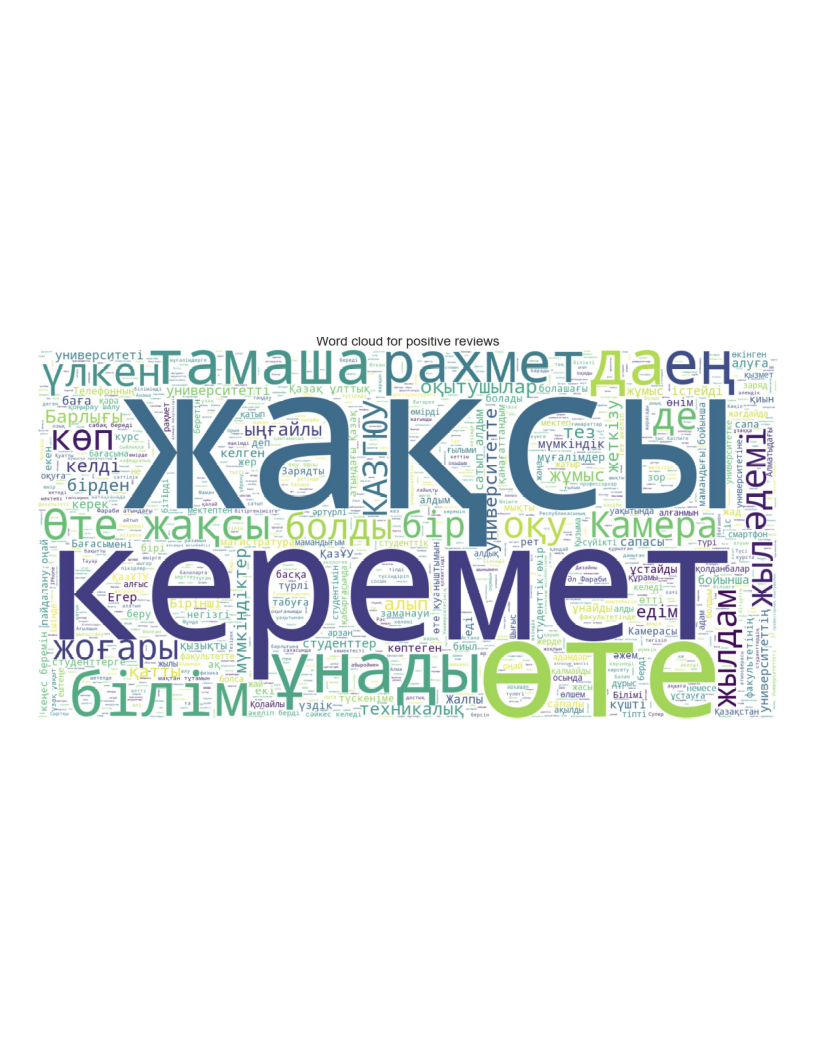
\includegraphics[width=0.8\textwidth]{media/ict/image9}
	\caption*{Figure 1 - Word cloud of positive comments}
\end{figure}

\begin{figure}[H]
	\centering
	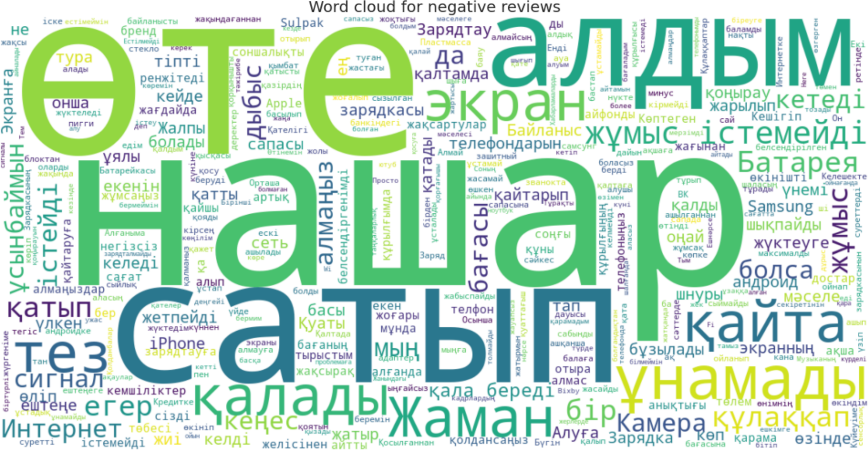
\includegraphics[width=0.8\textwidth]{media/ict/image10}
	\caption*{Figure 2 - Word cloud of negative comments}
\end{figure}

\begin{multicols}{2}
Figure 3 shows the bigram analysis of the comments. From this analysis,
we can see exactly which phrases generate positive and negative
feedback. In our case, "excellent", "best", "bought", "liked" and so on.
bigrams were most often used in positive comments, while bigrams such as
"do not recommend", "doesn' t work", "worst" were most
often used in describing negative comments.

\emph{Feature extraction from the processed data.} Feature extraction is
an important step involving the conversion of text data into vectors
that can be understood by machine learning algorithms. The following
methods are used to extract symbols from text data: one-hot encoding,
bag of words, term frequency - inverse document frequency (TF-IDF) and
word embeddings. In the work , term frequency - inverse document
frequency (TF-IDF) vectorizer was used to extract features. The TF-IDF
vectorizer is the most commonly used method for converting texts to
digital values. TF-IDF is a numerical statistic which indicates the
importance of a word for a document in a collection or corpus. It is
calculated as a product of two components: Term Frequency (TF) and
Inverse Document Frequency (IDF) {[}17{]}.
\end{multicols}

\begin{figure}[H]
	\centering
	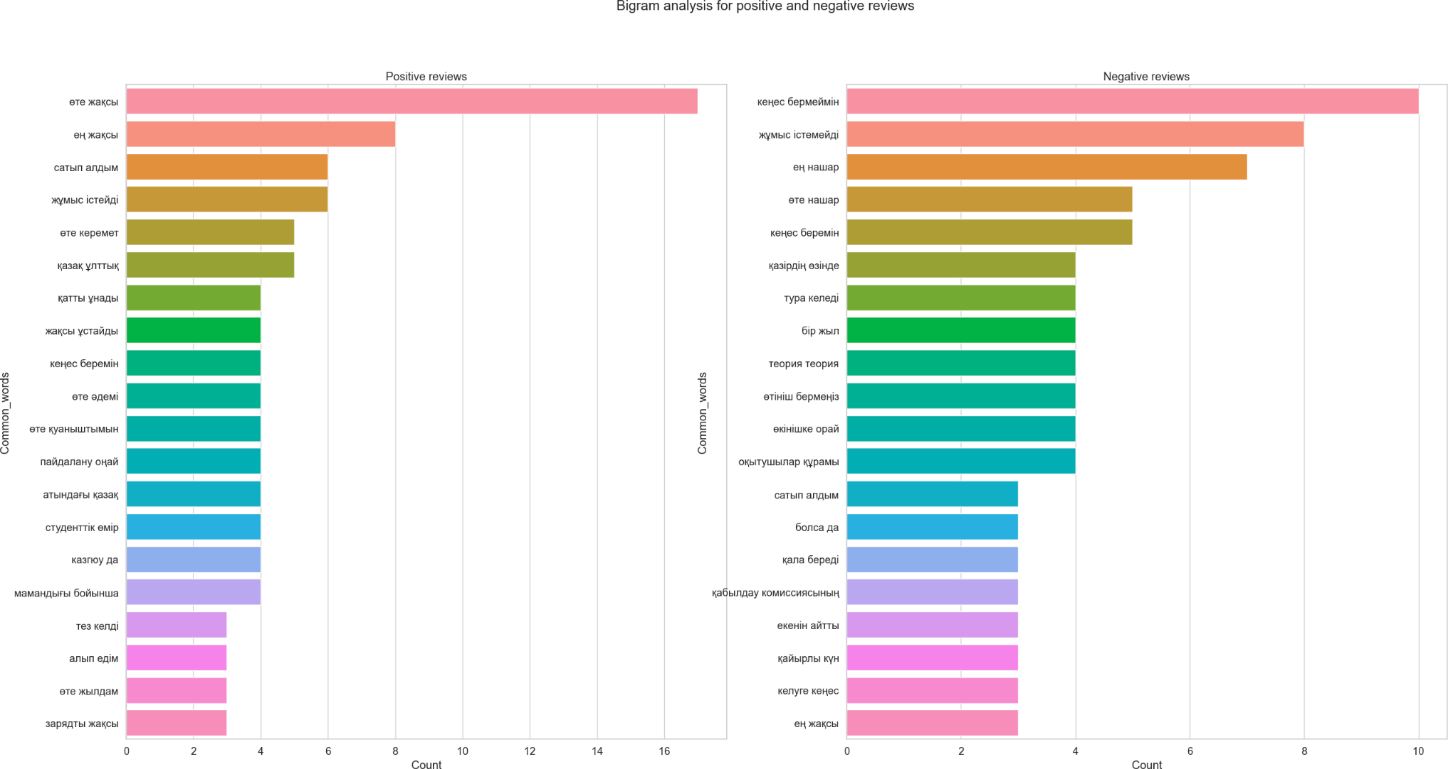
\includegraphics[width=0.9\textwidth]{media/ict/image11}
	\caption*{Figure 3 - Bigram analysis for negative and positive reviews}
\end{figure}

\begin{multicols}{2}
A matrix of numeric vectors was created by applying the TF-IDF formula
on the corpus of documents. Each row of the matrix represents a
document, and each column represents a unique word in the corpus. The
resulting matrix was fed as input to various machine learning algorithms
for sentiment analysis. The TF-IDF vectorizer is a powerful tool for
feature extraction from textual data in sentiment analysis because it
shows both the importance of words in a document and their rarity in the
corpus. This helps improve the accuracy and efficiency of machine
learning models for sentiment analysis.

\emph{Implementation of sentimental data analysis with machine learning
algorithms.} Conducting sentimental analysis of reviews consists of
several steps. The sequence of steps is shown in Figure 4. The first
analyzed data is pre-processed. Then, the textual data in the training
and test sets were transformed into numerical feature vectors based on
the TF-IDF representation. This transformation allows machine learning
algorithms to work efficiently with textual data, as they typically
require numerical input.
\end{multicols}


\begin{figure}[H]
	\centering
	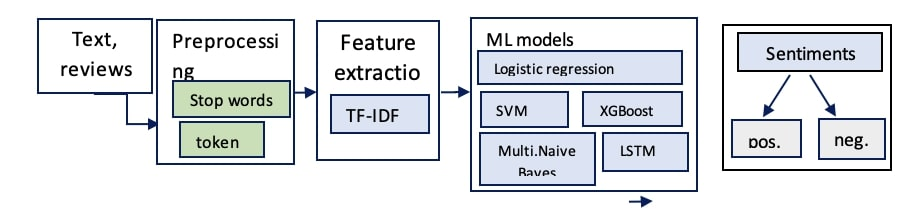
\includegraphics[width=0.6\textwidth]{media/ict/image10.2}
	\caption*{Figure 4 - Steps of processing text data using machine learning}
\end{figure}

The data set was divided into training and test sets using the
train\_test\_split function of the scikit-learn library. The Test\_size
parameter was set to 0.2, that is, 20\% of this data was used for
testing, and 80\% was used for training. Using the converted TF-IDF
data, a version of the LogisticRegression class was developed, which was
displayed by the logistic regression algorithm. As the logistic
regression algorithm and target labels are trained through the training
data, the identification method adjusts the sample parameters to find
the best fit for the given data. The accuracy, classification
calculation, and confusion matrix for estimating sample performance are
as follows (Figure 5):

\begin{figure}[H]
	\centering
	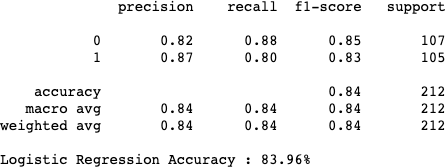
\includegraphics[width=0.8\textwidth]{media/ict/image12}
	\caption*{Figure 5 - Accuracy of logistic regression algorithm}
\end{figure}

And to use the Multinomial Naive Bayes model, the sklearn.naive\_bayes
function was used. A Multinomial Naive Bayes classifier was instantiated
and trained on the training data represented by the TF-IDF vectorized
feature matrix and the corresponding feature matrix. The features of the
test data were predicted using the trained MNB classifier. The accuracy
score was calculated by comparing the predicted signs with the real
signs (accuracy indicators are shown in Figure 6).

\begin{figure}[H]
	\centering
	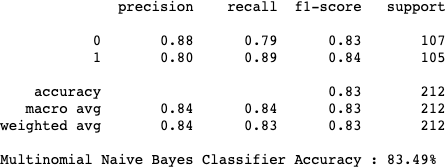
\includegraphics[width=0.8\textwidth]{media/ict/image13}
	\caption*{Figure 6-Accuracy of Multinomial Naive Bayes model}
\end{figure}

In addition, Linear SVM and XGboost models of machine learning are also
tested. Their results are lower than logistic regression (Linear
SVM-79.25\%, Xgboost-80.1\%).

\emph{Implementation of sentimental data analysis with deep learning
algorithms.} In order to use the Recurrent Neural Network (RNN) method,
it is necessary to build a vocabulary. This is an efficient lookup table
where each unique word in the data set has a corresponding index
(integer). Based on the reviews, the following dictionary was compiled:

\emph{{[}«Керемет телефон екен», «Маған ұнады әдемі», «Қуаты өте ұзаққа
шыдайды»{]} → vocabulary \{«\textless unk\textgreater»:0, «әдемі»:1,
«екен»:2, «керемет»:3, «маған»:4, «телефон»:5, «қуат»: 6, «ұзаққа»:7,
«ұнады»:8, «өте»:9, «шыдайды»:10, «pad»:11\}}

Then, using a dictionary, we assigned indexes to the text data in the
test set, replacing each word in the data with the corresponding index
in the dictionary. In this step, the textual data is converted into
numerical representations that can be used as input to the RNN. The
following conversion is obtained:

\emph{{[}«Керемет телефон екен», «Маған ұнады әдемі», «Қуаты өте ұзаққа
шыдайды»{]} → vocabulary \{«\textless unk\textgreater»:0, «әдемі»:1,
«екен»:2, «керемет»:3, «маған»:4, «телефон»:5, «қуат»: 6, «ұзаққа»:7,
«ұнады»:8, «өте»:9, «шыдайды»:10, «pad»:11\} → \{\{«Керемет телефон
екен»: {[}3 5 2 11{]}\}, \{«Маған ұнады әдімі»: {[}4 8 1 11{]}\},
\{«Қуат өте ұзаққа шыдайды»: {[}6 9 7 10{]}\}\}}

Each index is used to create a vector for each word. One-hot vector is a
vector whose size is the total number of unique words in the dictionary,
where only one element is 1, and all other elements are 0 (Figure 7).
Tourch libbrary was used for this task.

\begin{figure}[H]
	\centering
	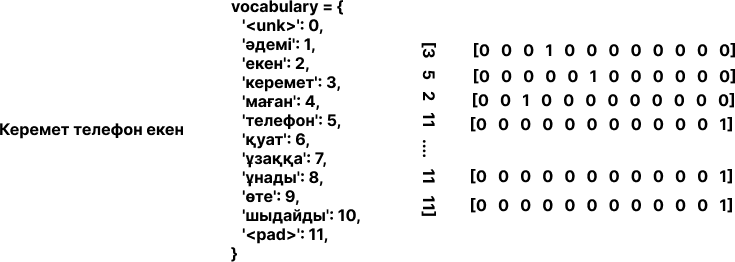
\includegraphics[width=0.8\textwidth]{media/ict/image14}
	\caption*{Figure 7-One-hot vector}
\end{figure}

An embedding layer was used to transform a one-hot vector into a dense
embedding vector. The model constructor consists of the size of the
input dictionary, the number of unique tokens in the textual data
(input\_dim), the dimensionality of the embedding vectors representing
the input tokens (embedding\_dim), the number of units in the hidden
state of the LSTM (hidden\_dim), the dimensionality of the output
representing the sentiment prediction (output\_dim). The implementation
of the model is presented in Figure 8.

\begin{figure}[H]
	\centering
	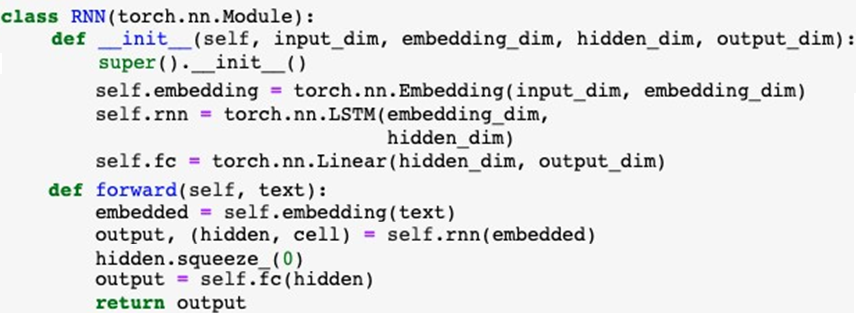
\includegraphics[width=0.8\textwidth]{media/ict/image15}
	\caption*{Figure 8 - RNN model creation}
\end{figure}

In addition, the torch.nn.Embedding module was created, which is
responsible for learning and matching input tokens with dense embedding
vectors. And the torch.nn.LSTM module was built to implement the long
LSTM layer. This module takes embedded input as input and processes the
serial information to generate hidden states. Next, a torch.nn.Linear
module was created which maps the last hidden state to the output
dimension responsible for sentiment prediction.

The Forward method is responsible for the forward movement of the model.
It accepts text as input text data. An embedded tensor is obtained by
passing the input text through an embedding layer, performing a search
to transform the input tokens into dense vector representations. The
embedded tensor is then passed through the RNN layer and returns the
(hidden, cell) values containing the output features of the LSTM for
each time step and the final hidden state of the LSTM. The latent tensor
is filtered along the first dimension to remove the extra dimension
added by the LSTM.

Next, the created model was trained. This process consisted of 10
stages. Logs the training progress, updating model parameters based on
calculated gradients. It also evaluates the performance of the model on
the training and validation sets after each phase. Finally, 60\%
accuracy was obtained from model training. 60\% is not considered a good
result, so ways to improve its accuracy rate were considered.

To increase the accuracy of the model, various modifications were made
to the LSTM algorithm, including the embedded use of the packed padded
sequences method, which gave good results. Important aspects of packed
padded sequences are defined (example implementation code is shown in
Figure 9):

\begin{itemize}
\item
  Efficient computation: Stacked filled sequences allow for more
  efficient computation during training and inference. In RNNs, input
  sequences are usually processed in parallel in a small batch. Filled
  circuits avoid unnecessary computations on filled elements, resulting
  in faster training and reduced inference time.
\item
  Memory efficiency: padded circuits increase memory requirements
  because they introduce a significant number of padded elements. By
  wrapping strings, filled elements are effectively masked, reducing the
  memory footprint and optimizing memory usage.
\item
  Improved model performance: Overloaded circuits can negatively impact
  model performance by introducing noise and unnecessary calculations.
\end{itemize}

\begin{figure}[H]
	\centering
	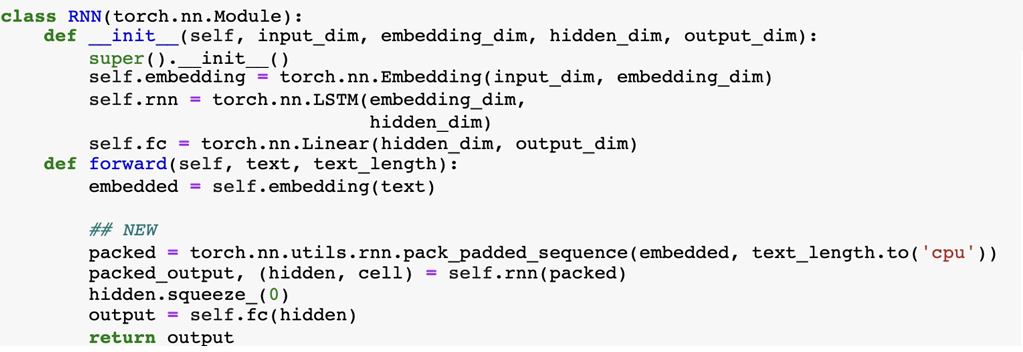
\includegraphics[width=0.8\textwidth]{media/ict/image16}
	\caption*{Figure 9 - Improved LSTM algorithm code}
\end{figure}

This function creates a boxed sequence object which represents sequences
without padding tokens. Using this method, 84\% accuracy was achieved.

\emph{Discussion of results.} Let' s look at which method
gives better results by comparing the results of sentimental analysis
made using Logistic Regression, Multinomial Naive Bayes, Liner SVM,
XGBoost, Long short-term memory (LSTM), LSTM-pack sequence learning
methods to improve LSTM on collected Kazakh comments. Table 1 shows the
results of the above-mentioned models and algorithms evaluation
experiment

\begin{table}[H]
\caption*{Table 1 - Results of algorithm}
\centering
\begin{tabular}{|l|l|l|}
\hline
№ & Algorithm name              & Accuracy \\ \hline
1 & Logistic regression         & 83.96\%  \\ \hline
2 & Multinomial Naive Bayes     & 83.49\%  \\ \hline
3 & Linear SVM                  & 79,25\%  \\ \hline
4 & XGboost                     & 80,1\%   \\ \hline
5 & LSTM                        & 60.00\%  \\ \hline
6 & Improved LSTM               & 84.12\%  \\ \hline
\end{tabular}
\end{table}

\begin{multicols}{2}
Due to the lack of a large collection of data, machine learning methods
have shown that they do not give more accurate results. A logistic
regression algorithm can be effective if there is low-dimensional data
and their capability is linearly distributed, but a large data set is
required to achieve good results. Although the LSTM model showed only 60
percent accuracy, it increased its accuracy using the packed packed
sequences method and achieved better results than everyone else. The
LSTM model has shown poor performance on very little data. When we
increased the number of reviews from 500 to 1500, we noticed a
improvement in the result.

{\bfseries Conclusion.} This paper is devoted to the study of ways of
sentimental analysis of Kazakh language reviews. The introduction of the
article explains sentimental analysis and gives citations for its
importance. The paper considered lexicon (rule) based methods, machine
learning based methods and deep learning methods as methods of
sentimental data analysis. Among them, we differentiated the
possibilities of determining the mood in Kazakh-language opinions using
methods based on machine learning and deep learning methods, which are
currently being extensively researched and are well used in practical
developments.

Kazakh-language reviews used in sentimental analysis were collected from
Kaspi online-market, nur.kz and 2GIS. Collected opinions were subjected
to initial processing such as preliminary processing and preparation of
the data set, analysis (review) of the processed data set, extraction of
features from the processed data. Further, the prepared data were
sentimentally analyzed using Logistic regression, Multinomial Naive
Bayes, Linear SVM, Xgboost and deep learning LSTM models of machine
learning and the accuracy indicators of the obtained results were
determined. After all samples were analyzed, a comparative analysis of
their accuracy indicators was performed. Comparative analysis showed
that the best result was the deep learning improved LSTM model
(accuracy-84.12\%), followed by the machine learning Logistic regression
model (accuracy-83.96\%).
\end{multicols}

\begin{center}
{\bfseries References}
\end{center}

\begin{references}
1. Bolshakova E.I., Voroncov K.V., Efremova N.E., Klyshinskij E.S.,
Lukashevich N.V., Sapin A.S. 

Avtomaticheskaya obrabotka tekstov na
estestvennom yazyke i analiz dannyh. - M.: Izd-vo NIU VShE, 2017. - 269
s. {[}in Russian{]}

2.~Pasolini, Roberto. Learning Methods and Algorithms for Semantic Text
Classification across Multiple Domains, {[}Dissertation thesis{]}. Alma
Mater Studiorum Università di Bologna. Dottorato di ricerca in
Ingegneria elettronica, informatica delle telecomunicazioni, 27 Ciclo.

DOI 10.6092/unibo/amsdottorato/7058.

3. Jingli Shi, Weihua Li, Quan Bai, Yi Yang, Jianhua Jiang.
Syntax-Enhanced Aspect-Based Sentiment Analysis with Multi-Layer
Attention // Neurocomputing. -2023.

DOI
\href{https://doi.org/10.1016/j.neucom.2023.126730}{10.1016/j.neucom.2023.126730}

4. Malliga Subramanian, Veerappampalayam Easwaramoorthy Sathiskumar, G.
Deepalakshmi, Jaehyuk Cho, G. Manikandan. A survey on hate speech
detection and sentiment analysis using machine learning and deep
learning models // Alexandria Engineering Journal. -- 2023. --Vol.
80(2). - P. 110-121.

DOI\href{http://dx.doi.org/10.1016/j.aej.2023.08.038}{10.1016/j.aej.2023.08.038}

5. Arwa A. Al Shamsi, Sherief Abdallah. Ensemble Stacking Model for
Sentiment Analysis of Emirati and Arabic Dialects // Journal of King
Saud University. -2023. -Vol. 35(8).

\href{https://doi.org/10.1016/j.jksuci.2023.101691}{DOI
10.1016/j.jksuci.2023.101691}

6. Meng Li, Yucheng Shi. Sentiment analysis and prediction model based
on Chinese government affairs microblogs // Heliyon. - 2023. DOI
\href{https://doi.org/10.1016/j.heliyon.2023.e19091}{10.1016/j.heliyon.2023.e19091}

7. Chetviorkin, I.; Loukachevitch, N. Evaluating Sentiment Analysis
Systems in Russian // In Proceedings of the 4th Biennial International
Workshop on Balto-Slavic Natural Language Processing, Sofia, Bulgaria,
8--9 August 2013; Association for Computational Linguistics . - Sofia,
Bulgaria, 2013. -P. 12--17.

8. Nugumanova A., Baiburin Ye., Alimzhanov Ye.. Sentiment Analysis of
Reviews in Kazakh With Transfer Learning Techniques // SIST 2022 - 2022
International Conference on Smart Information Systems and Technologies,
Proceedings, ISBN 978-166546790. - 2022.
DOI 10.1109/SIST54437.2022.9945811

9.~Karyukin Vladislav, Mutanov Galimkair, Mamykova Zhanl, Nassimova
Gulnar, Torekul Saule, Sundetova Zhanerke, Negri Matteo. On the
development of an information system for monitoring user opinion and its
role for the public // Journal of Big Data. -2022. - Vol. 9.
DOI 10.1186/s40537-022-00660-w

10. Narynov S.S., Zharmagambetov A.S.: On One Approach of Solving
Sentiment Analyis Task for Kazakh and Russian Languages Using Deep
Learning // International Conference on Computational Collective
Intelligence. - Springer, 2016. - Vol. 9876.
DOI 10.1007/978-3-319-45246-3\_51

11. Saraswathi N., Sasirooba T., Chakaravarthi S. Improving the accuracy
of sentiment analysis using a linguistic rule-based feature selection
method in tourism reviews // Measurement: Sensors. - 2023. - Vol. 29. -
DOI
\href{https://doi.org/10.1016/j.measen.2023.100888}{10.1016/j.measen.2023.100888}

12. Gulmira Bekmanova, Gaziza Yelibayeva, Saltanat Aubakirova, Nurgul
Dyussupova, Altynbek Sharipbay, Rozamgul Nyazova. Methods for analyzing
polarity of the Kazakh texts related to the terrorist threats //
Computational Science and Its Applications - ICCSA 2019. - P. 717-730.

DOI 10.1007/978-3-030-24289-3\_53

13. Gareth James, Daniela Witten, Trevor Hastie, Robert Tibshirani. An
Introduction to Statistical Learning with Applications in R // Springer
Science and Business Media. - New York, 2013.

DOI 10.1007/978-1-4614-7138-7

14. Dinara Gimadi, Richard Evans, Kiril Simov. Web-sentiment Analysis Of
Public Comments (Public Reviews) For Languages With Limited Resources
Such As The Kazakh Language. - 2021. 

DOI  10.26615/issn.2603-2821.2021\_010

15. Huseyn Hasanli , Burak Ordin , Samir Rustamov. Sentiment analysis on
twitter data for azerbaijani language // Journal of Modern Technology
and Engineering.-2019. - Vol.4. - No.2.
- P.109-121. 2019.

16.~Sebastian Raschka, Vahid Mirjalili. Python Machine Learning: Machine
Learning and Deep Learning with Python, scikit-learn, and TensorFlow 2.
- 2019. P. 770.

17. Ugo Erra, Sabrina Senatore, Fernando Minnella, Giuseppe Caggianese.
Approximate TF--IDF based on topic extraction from massive message
stream using the GPU // Information Sciences, January. - 2015. --Vol.
292. -P. 143-161. DOI10.1016/j.ins.2014.08.062
\end{references}

\begin{authorinfo}
\hspace{1em}\emph{{\bfseries Information about the authors}}

Mukazhanov N. K. - doctor Ph.D., associate professor, Satbayev
University, Almaty, Kazakhstan, 

е-mail:
\href{mailto:n.mukazhanov@satbayev.university}{\nolinkurl{n.mukazhanov@satbayev.university}};

Cherikbayeva L.Sh. - doctor Ph.D., Al-Farabi Kazakh National University,
Almaty, Kazakhstan, 

е-mail:
\href{mailto:cherikbayeva.lyailya@gmail.com}{\nolinkurl{cherikbayeva.lyailya@gmail.com}};

Kasenkhan A.M. -- doctor Ph.D., Satbayev University, Almaty, Kazakhstan,
e-mail:
\href{mailto:a.kassenkhan@satbayev.university}{\nolinkurl{a.kassenkhan@satbayev.university}};

Alibieva Zh.M. - doctor Ph.D., associate professor, Satbayev University,
Almaty, Kazakhstan,

е-mail:
\href{mailto:zh.alibiyeva@satbayev.university}{\nolinkurl{zh.alibiyeva@satbayev.university}};

Turdalyuly M. - doctor Ph.D., associate professor, International
Engineering and Technological University, Almaty, Kazakhstan, е-mail:
m.turdalyuly@gmail.com

\hspace{1em}\emph{{\bfseries Сведения об авторах}}

Мукажанов Н.К. - доктор Ph.D, ассоциированный профессор, Satbayev
University, Алматы, Казахстан, 

е-mail:
\href{mailto:n.mukazhanov@satbayev.university}{\nolinkurl{n.mukazhanov@satbayev.university}};

Черикбаева Л.Ш. - доктор Ph.D, Казахский национальный университет им.
Аль-Фараби, Алматы, Казахстан, е-mail:
\href{mailto:cherikbayeva.lyailya@gmail.com}{\nolinkurl{cherikbayeva.lyailya@gmail.com}};

Қасенхан А.М - доктор Ph.D, Satbayev University, Алматы, Казахстан,
e-mail:
\href{mailto:a.kassenkhan@satbayev.university}{\nolinkurl{a.kassenkhan@satbayev.university}};

Алибиева Ж.М. - доктор Ph.D, ассоциированный профессор, Satbayev
University, Алматы, Казахстан, 

е-mail:
\href{mailto:zh.alibiyeva@satbayev.university}{\nolinkurl{zh.alibiyeva@satbayev.university}};

Тұрдалыұлы М. - доктор Ph.D, ассоциированный профессор, Международный
инженерно-технологический университет, Алматы, Казахстан, е-mail:
m.turdalyuly@gmail.com
\end{authorinfo}
